\section{Auswertung}
\label{sec:Auswertung}

% % Examples
% \begin{equation}
%   U(t) = a \sin(b t + c) + d
% \end{equation}
%
% \begin{align}
%   a &= \input{build/a.tex} \\
%   b &= \input{build/b.tex} \\
%   c &= \input{build/c.tex} \\
%   d &= \input{build/d.tex} .
% \end{align}
% Die Messdaten und das Ergebnis des Fits sind in Abbildung~\ref{fig:plot} geplottet.
%
% %Tabelle mit Messdaten
% \begin{table}
%   \centering
%   \caption{Messdaten.}
%   \label{tab:data}
%   \sisetup{parse-numbers=false}
%   \begin{tabular}{
% % format 1.3 bedeutet eine Stelle vorm Komma, 3 danach
%     S[table-format=1.3]
%     S[table-format=-1.2]
%     @{${}\pm{}$}
%     S[table-format=1.2]
%     @{\hspace*{3em}\hspace*{\tabcolsep}}
%     S[table-format=1.3]
%     S[table-format=-1.2]
%     @{${}\pm{}$}
%     S[table-format=1.2]
%   }
%     \toprule
%     {$t \:/\: \si{\milli\second}$} & \multicolumn{2}{c}{$U \:/\: \si{\kilo\volt}$\hspace*{3em}} &
%     {$t \:/\: \si{\milli\second}$} & \multicolumn{2}{c}{$U \:/\: \si{\kilo\volt}$} \\
%     \midrule
%     1.7 & 10 \\
2.3 & 20 \\
3.5 & 30 \\
4.4 & 40 \\

%     \bottomrule
%   \end{tabular}
% \end{table}
%
% % Standard Plot
% \begin{figure}
%   \centering
%   \includegraphics{build/plot.pdf}
%   \caption{Messdaten und Fitergebnis.}
%   \label{fig:plot}
% \end{figure}
%
% 2x2 Plot
% \begin{figure*}
%     \centering
%     \begin{subfigure}[b]{0.475\textwidth}
%         \centering
%         \includegraphics[width=\textwidth]{Abbildungen/Schaltung1.pdf}
%         \caption[]%
%         {{\small Schaltung 1.}}
%         \label{fig:Schaltung1}
%     \end{subfigure}
%     \hfill
%     \begin{subfigure}[b]{0.475\textwidth}
%         \centering
%         \includegraphics[width=\textwidth]{Abbildungen/Schaltung2.pdf}
%         \caption[]%
%         {{\small Schaltung 2.}}
%         \label{fig:Schaltung2}
%     \end{subfigure}
%     \vskip\baselineskip
%     \begin{subfigure}[b]{0.475\textwidth}
%         \centering
%         \includegraphics[width=\textwidth]{Abbildungen/Schaltung4.pdf}    % Zahlen vertauscht ... -.-
%         \caption[]%
%         {{\small Schaltung 3.}}
%         \label{fig:Schaltung3}
%     \end{subfigure}
%     \quad
%     \begin{subfigure}[b]{0.475\textwidth}
%         \centering
%         \includegraphics[width=\textwidth]{Abbildungen/Schaltung3.pdf}
%         \caption[]%
%         {{\small Schaltung 4.}}
%         \label{fig:Schaltung4}
%     \end{subfigure}
%     \caption[]
%     {Ersatzschaltbilder der verschiedenen Teilaufgaben.}
%     \label{fig:Schaltungen}
% \end{figure*}
\subsection{Bestimmung der Schallgeschwindigkeit in Acryl mittels Impuls-Echo-Verfahren}
Die Messung der einzelnen Zylinder mittels Schieblehre ergibt die Zylinderhöhen
\begin{align*}
  h_1 &= \SI{61.5}{\milli\metre}, \\
  h_2 &= \SI{80.55}{\milli\metre}, \\
  h_3 &= \SI{102.1}{\milli\metre}, \\
  h_4 &= \SI{120.5}{\milli\metre}, \\
  h_5 &= \SI{31.3}{\milli\metre}.
\end{align*}
Die Durchführung eines Impuls-Echo-Verfahren ergibt die in Tabelle \ref{tab:0} dargestellten Laufzeiten $\increment t$ zu den jeweiligen Zylinderhöhen $h$.
Hierbei werden zunächst alle Zylinder einzeln und zum Schluss zwei Kombinationen aus $h_5$ und $h_1$ bzw. $h_2$ betrachtet.
Aus dem Weg-Zeit-Gesetz wird somit die jeweilige Geschwindigkeit des Impulses berechnet, wobei aufgrund der Reflextion die doppelte Weglänge berücksichtigt werden muss.
  \input{build/Tabelle_0_texformat.tex}
Die Bestimmung der Mittelwertes nach Formel \eqref{eq:std_mean} sowie die Bestimmung des Fehlers nach Formel \eqref{eq:std} ergibt somit eine gemittelte Schallgeschwindigkeit in Acryl von
\begin{align*}
  c_{\text{acryl,e}} &= \input{build/c_acryl_1.tex}.\\
\end{align*}

Die genauere Betrachtung der ersten Messung ergibt eine Amplitude des ersten Peaks von
\begin{align*}
  U_1 = \SI{1.214}{\volt}

\end{align*}
sowie eine Amplitude des zweiten Peaks von
\begin{align*}
  U_2 = \SI{1.105}{\volt}
.
\end{align*}
Die Peaks werden zu den Laufzeiten
\begin{align*}
  t_1 = \SI{1.3}{\micro\second}

\end{align*}
beziehungsweise
\begin{align*}
  t_2 = \SI{46.2}{\micro\second}

\end{align*}
gemessen.
Hieraus ergibt sich die zuvor in Tabelle \ref{tab:0} angegebene Laufzeitdifferenz.
Bei Eingabe der berechneten Schallgeschwindigkeit in das Auswertungsprogramm ergibt sich für die Tiefenmessung exakt die mit der Schieblehre gemessene Länge des Zylinders, was die Funktion des Programmes bestätigt. %duh

\subsubsection{Ausgleichsrechnung zur Bestimmung des systematischen Fehlers}
Aufgrund der endlichen Dicke der Anpassungsschicht der Sonde tritt ein systematischer Fehler auf.
Um diesen zu ermitteln, werden die gemessenen Weglängen gegen die halbierten Laufzeiten aufgetragen und ein linearer Fit durchgeführt.
Der Grund der halbierten Laufzeiten ist wiederum die effektive doppelte Weglänge, die zurückgelegt werden muss.
Diese wird in Python mit Numpy mittels der Methode der kleinsten Quadrate durchgeführt.
Es ergibt sich der in Abbildung \ref{fig:plot1} dargestellte Graph.
\begin{figure}
  \centering
  \includegraphics{build/ausgleich.pdf}
  \caption{Ausgleichsrechnung zur Bestimmung der Dicke der Anpassungsschicht.}
  \label{fig:plot1}
\end{figure}
Die ermittelten Fitparameter sind dabei
\begin{align*}
  m &= \input{build/parameter_a.tex} \\
  b &= \input{build/parameter_b.tex}.
\end{align*}
Die Steigung lässt sich hierbei identifizieren als Wert für die Schallgeschwindigkeit in Acryl, der Achsenabschnitt beschreibt den systematischen Fehler, bzw. die Dicke der Anpassungsschicht.

\subsection{Bestimmung der Schallgeschwindigkeit in Acryl mittels Durchschallungs-Methode}
Für die Messungen mit der Durchschallungs-Methode ergeben sich die Werte aus Tabelle \ref{tab:1}, wobei die Computer-Software die Messung für größere Zylinder nicht möglich gemacht hat.
  \input{build/Tabelle_1_texformat.tex}
Mit Hilfe dieser wird die gemittelte Schallgeschwindigkeit in Acryl auf
\begin{align*}
  c_{\text{acryl,d}} &= \input{build/c_acryl_2.tex}\\
\end{align*}
bestimmt.

\subsection{Bestimmung des Abschwächungskoeffizienten von Acryl}
Aus den Werten der Intensitätspeaks und Laufzeiten der Echo-Impuls Messung kann der Schwächungskoeffizient $\alpha$ nach Gleichung \ref{gl:1} auf die Weise
\begin{equation}
  \alpha = \frac{\ln{\frac{U_1}{U_2}}}{t_1-t_2}
\end{equation}
berechnet werden.
Somit ergibt sich
\begin{align*}
  \alpha &= \input{build/alpha.tex}.\\
\end{align*}

\subsection{Bestimmung der Maße der Platten mittels FFT und Cepstrum}
Das gemessene Fourierspektrum ist in Abbildung \ref{fig:fft} dargestellt, das Cepstrum in Abbildung \ref{fig:cep}.
\begin{figure}
  \centering
  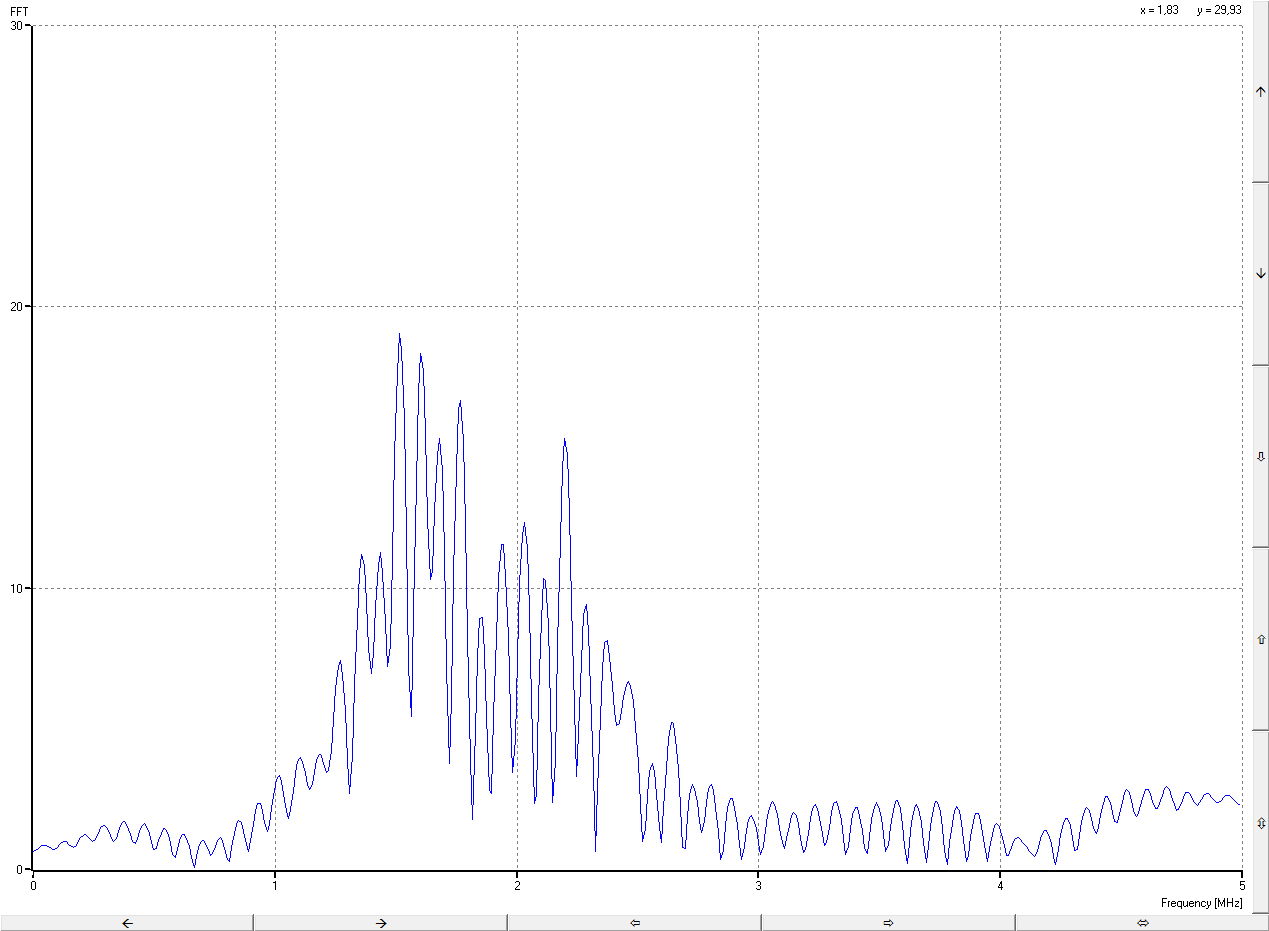
\includegraphics[height=10cm]{messdaten/fourier.png}
  \caption{Fouriertrasformation der Messung.}
  \label{fig:fft}
\end{figure}

\begin{figure}
  \centering
  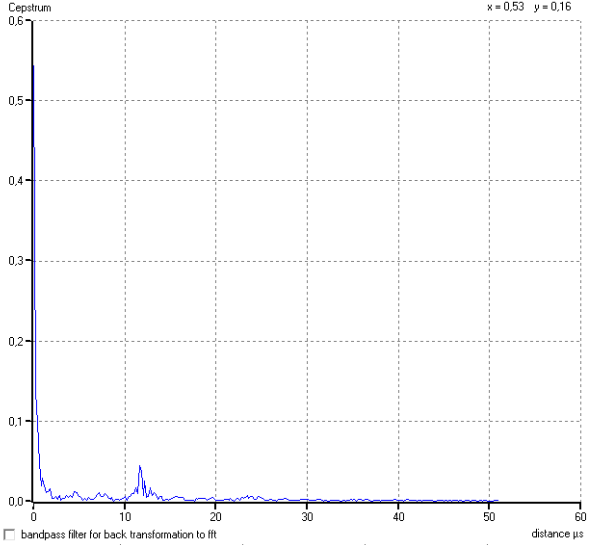
\includegraphics[height=10cm]{messdaten/cepstrum.png}
  \caption{Cepstrum der Messung.}
  \label{fig:cep}
\end{figure}

Es fällt auf, dass die Abstände zwischen den Peaks im Fourierspektrum äquidistant sind.
Dementsprechend werden dem Spektrum die Frequenzen für sechs repräsentative Probepeaks entnommen, welche
\begin{align*}
  f_{1} &= \input{build/fft_1.tex}, \\
  f_{2} &= \input{build/fft_2.tex}, \\
  f_{3} &= \input{build/fft_3.tex}, \\
  f_{4} &= \input{build/fft_4.tex}, \\
  f_{5} &= \input{build/fft_5.tex}, \\
  f_{6} &= \input{build/fft_6.tex},
\end{align*}
sind.
Die Abstände der Frequenzen werden nach Formel \eqref{eq:std_mean} gemittelt.
Aus der entstandenen Frequenz sowie dem Literaturwert für die Schallgeschwindigkeit in Acryl erhält man eine Dicke von
\begin{align*}
  s_\text{Platten} = \input{build/s_probe.tex}.
\end{align*}
Zudem kann dem Cepstrum ein Peak entnommen werden, aus diesem erhält man analog eine Dicke von
\begin{align*}
  s_\text{Platten,cep} = \input{build/s_cep.tex}.
\end{align*}

\subsection{Biometrische Untersuchung eines Augenmodells}
Bei der Untersuchung des Augenmodells (\ref{abb:3}) mithilfe eines A-Scans ergibt sich das in Abbildung \ref{fig:messung_auge} dargestellte Ergebnis.
\begin{figure}
  \centering
  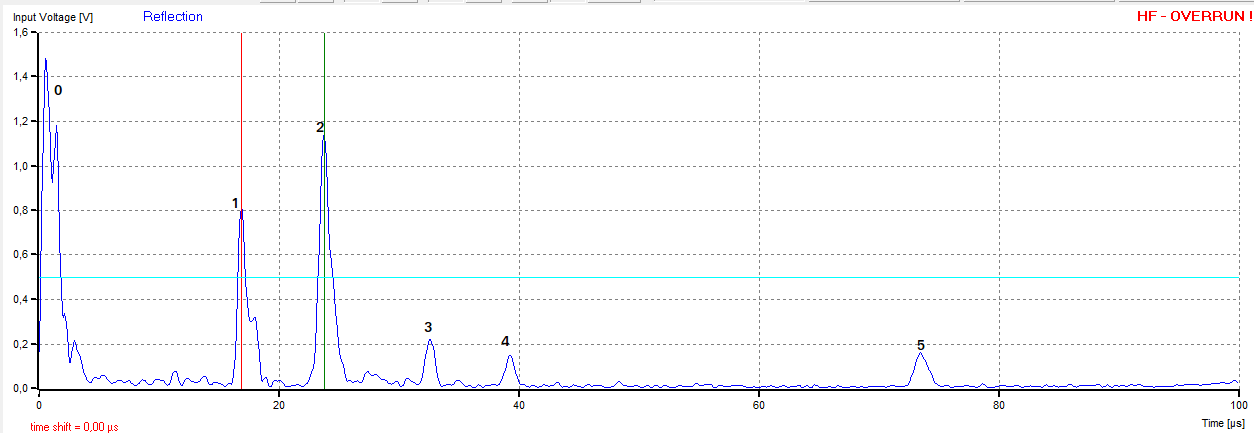
\includegraphics[height=5cm]{messdaten/auge_messung.png}
  \caption{Messung zur Untersuchung des Augenmodelles.}
  \label{fig:messung_auge}
\end{figure}
Die Intensitätsmaxima sind jeweils numeriert.
Das nullte Maximum wird als Eintritt in den ersten Glaskörper identifiziert, das erste und zweite Maximum als Reflexion an der linken bzw. an der rechten Seite der Linse.
Das dritte und vierte Maximum resultieren aus Mehrfachreflexionen an der Linse.
Zuletzt entspricht das fünfte Maximum der Reflexion an der Retina.
Bei der Berechnung der Weglängen sind die unterschiedlichen Schallgeschwindigkeiten im Glaskörper von
\begin{align*}
  c_\text{gk} &= \input{build/c_gk.tex}
\end{align*}
sowie in der Linse von
\begin{align*}
  c_\text{linse} &= \input{build/c_linse.tex}.
\end{align*}
Es ergeben sich hieraus die Abstände
\begin{align*}
  s_{0,1} &= \input{build/s_12.tex}, \\
  s_{1,2} &= \input{build/s_23.tex}, \\
  s_{2,5} &= \input{build/s_36.tex}. \\
\end{align*}
Hierbei entspricht $s_{0,1}$ dem Durchmesser des vorderen Glaskörpers, $s_{1,2}$ der Linsendicke sowie $s_{2,5}$ dem Durchmesser des hinteren Glaskörpers.
